\chapter{Appendix for Aromaticity as a Guide to Planarity in Conjugated Molecules and Polymers}

\section{Different Length Polymer Chains}\label{sec:aroma_diff_len_poly}
\begin{figure}[hbt!]
    \centering
    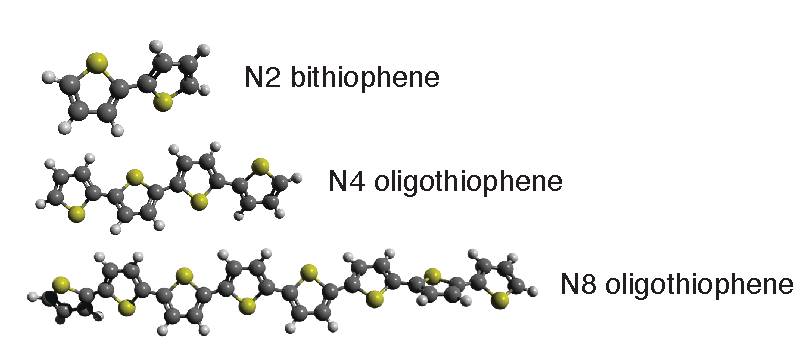
\includegraphics{figures/append_aroma/p_chains_graphic_copy.pdf}
    \caption[Different Length Thiophene Oligomers]{Different length oligomers of thiophene.}
    \label{fig:p_chains}
\end{figure}

\subsection{Comparison of Torsion Potentials}
\begin{figure}[hbt!]
    \centering
    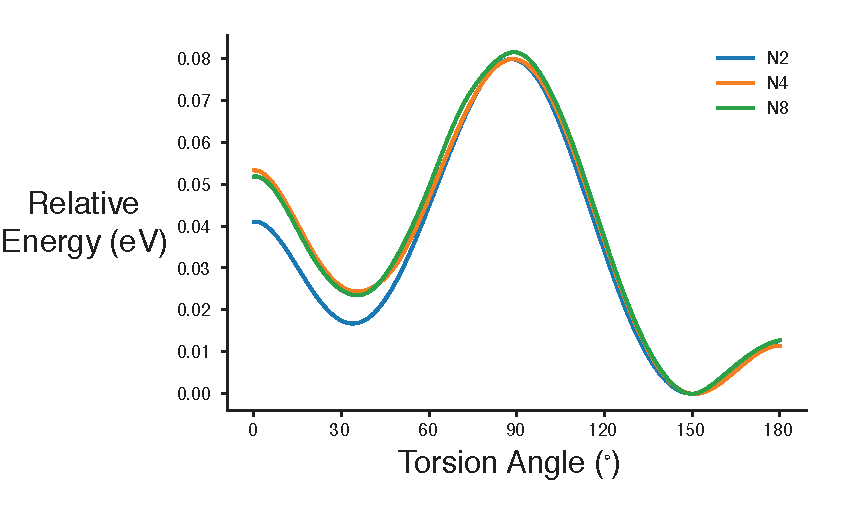
\includegraphics{figures/append_aroma/p_tor_compare_copy.pdf}
    \caption[Torsion Potential of Different Length Thiophene Oligomers]{The torsion potential of N2, N4, and N8 thiophene oligomers. All calculations were performed using the $\omega$B97x-D functional. The N2 torsion potential was calculated with the def2-TZVPP basis set, while N4 and N8 utilized the 6-31++G** \cite{Hehre1972} basis set to reduce to the computational cost. The deviation of N2 from both N4 and N8 between 0 and 50\textdegree \ is likely due to the different basis sets employed.}
    \label{fig:p_tor_compare}
\end{figure}

\clearpage
\subsection{Comparison of NICS Aromaticity}
\begin{figure}[hbt!]
    \centering
    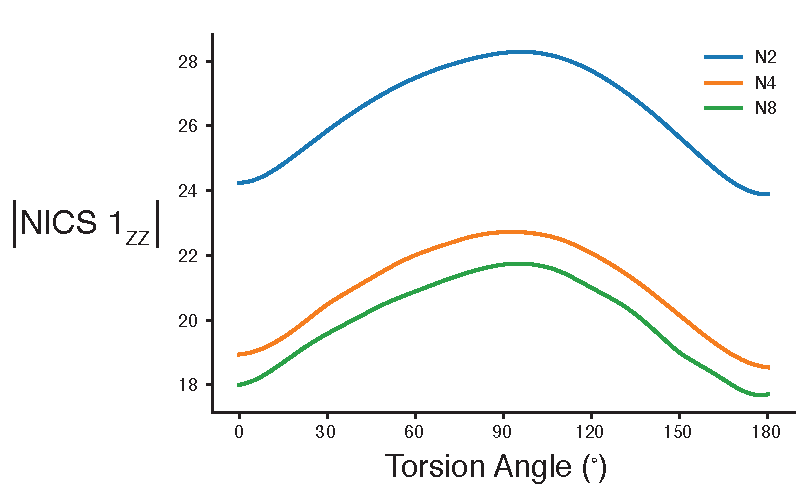
\includegraphics{figures/append_aroma/p_NICS_compare_copy.pdf}
    \caption[Aromaticity of Different Length Thiophene Oligomers ]{N2, N4, and N8 absolute NICS $1_{ZZ}$ values as a function of torsion angle. The magnitude of NICS values decrease with chain length, and we expect that the values will converge once a certain chain length is reached. While the magnitude decreases the overall trend as a function of torsion angle is consistent, which allows N2 to represent larger chains.}
    \label{fig:p_NICS_compare}
\end{figure}

\clearpage
\section{Comparision of MCI and NICS Aromaticity Values}\label{sec:aroma_mci_nics_comp}

\subsection{BT}
\begin{figure}[hbt!]
    \centering
    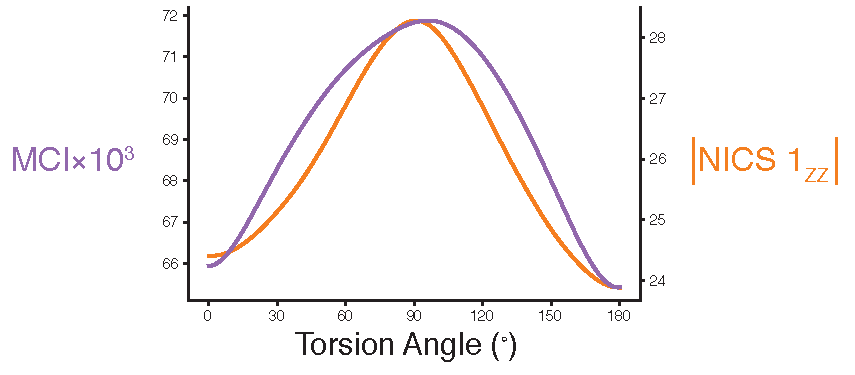
\includegraphics{figures/append_aroma/pt_aroma_compare_copy.pdf}
    \caption[Comparison of the Aromaticity Indexes MCI and NICS for BT]{Comparison of the aromaticity indexes MCI and NICS for BT.}
    \label{fig:pt_aroma_compare}
\end{figure}

\subsection{hBT}
\begin{figure}[hbt!]
    \centering
    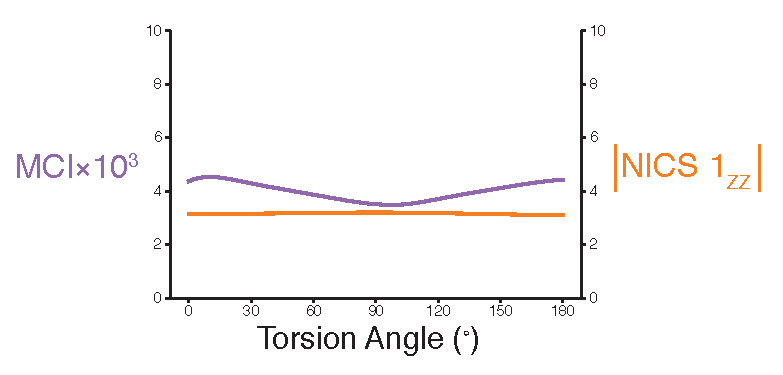
\includegraphics{figures/append_aroma/hpt_aroma_compare_copy.pdf}
    \caption[Comparison of the Aromaticity Indexes MCI and NICS for hBT]{Comparison of the aromaticity indexes MCI and NICS for hBT.}
    \label{fig:hpt_aroma_compare}
\end{figure}

\clearpage
\subsection{F2-BT}
\begin{figure}[hbt!]
    \centering
    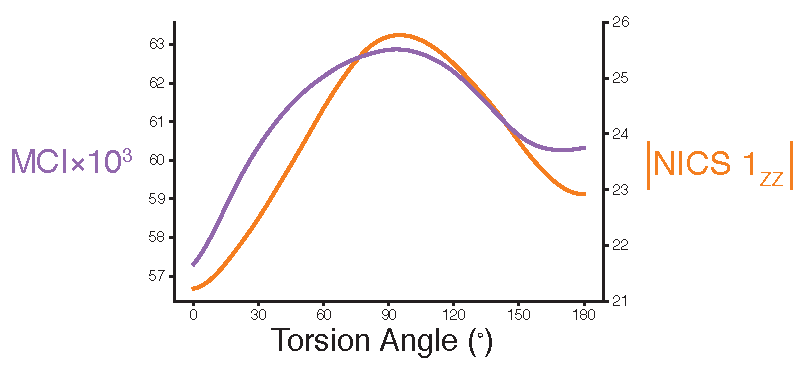
\includegraphics{figures/append_aroma/pt_f2_aroma_compare_copy.pdf}
    \caption[Comparison of the Aromaticity Indexes MCI and NICS for F2-BT]{Comparison of the aromaticity indexes MCI and NICS for F2-BT.}
    \label{fig:pt_f2_aroma_compare}
\end{figure}


\subsection{BEDOT}
\begin{figure}[hbt!]
    \centering
    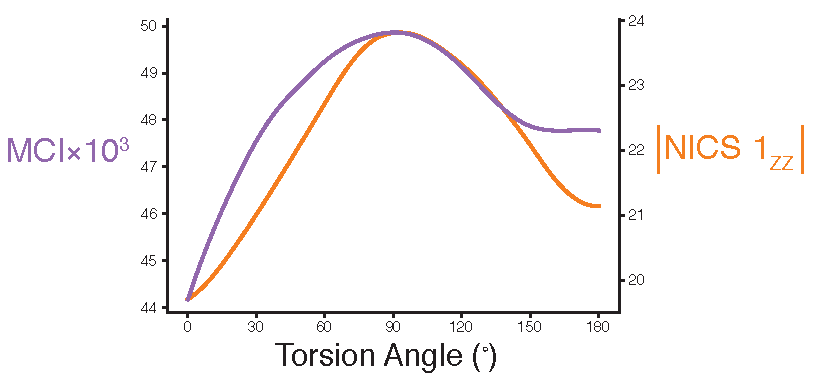
\includegraphics{figures/append_aroma/pedot_aroma_compare_copy.pdf}
    \caption[Comparison of the Aromaticity Indexes MCI and NICS for BEDOT]{Comparison of the aromaticity indexes MCI and NICS for BEDOT.}
    \label{fig:pedot_aroma_compare}
\end{figure}

\clearpage
\section{Through-space Interactions}\label{sec:aroma_ts}
\subsection{\texorpdfstring{H $\cdots$ S}{HS}}
\begin{figure}[hbt!]
    \centering
    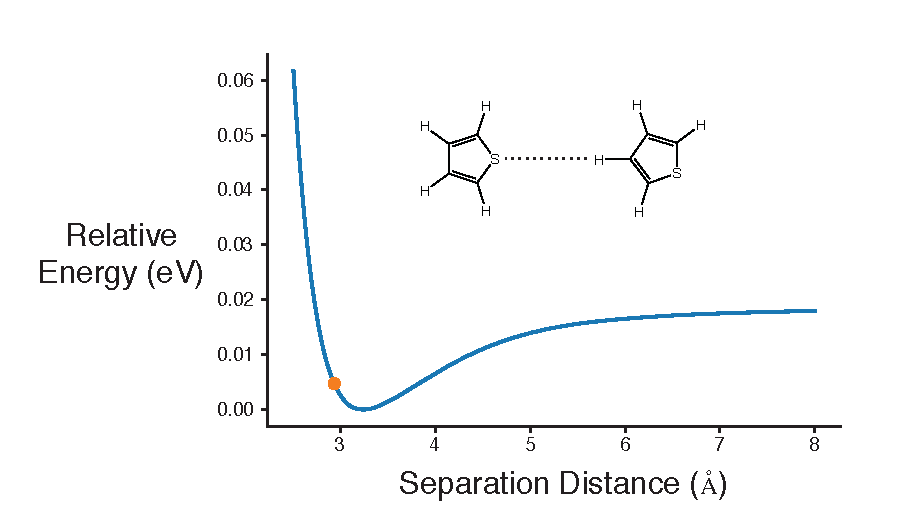
\includegraphics{figures/append_aroma/ts_t_t_copy.pdf}
    \caption[\texorpdfstring{H $\cdots$ S}{HS} Through-space Calculation]{A potential energy scan of the interatomic separation distance between a hydrogen and a sulfur atom on thiophene molecules. The orange dot represents the relaxed H $\cdots$ S distance on a trans (180\textdegree) BT molecule. This indicates that the H $\cdots$ S through-space interaction is marginally repulsive in trans BT. It is noteworthy that the repulsive energy is small compared to the torsional barrier present at 180\textdegree \ in BT (a factor of $\sim$2.5), which in combination with the NCI analysis below demonstrate the minor role of sterics in determining planarity.}
    \label{fig:ts_t_t}
\end{figure}
\clearpage

\subsection{\texorpdfstring{H $\cdots$ S}{HSN} Noncovalent Interaction Analysis}
\begin{figure}[hbt!]
    \centering
    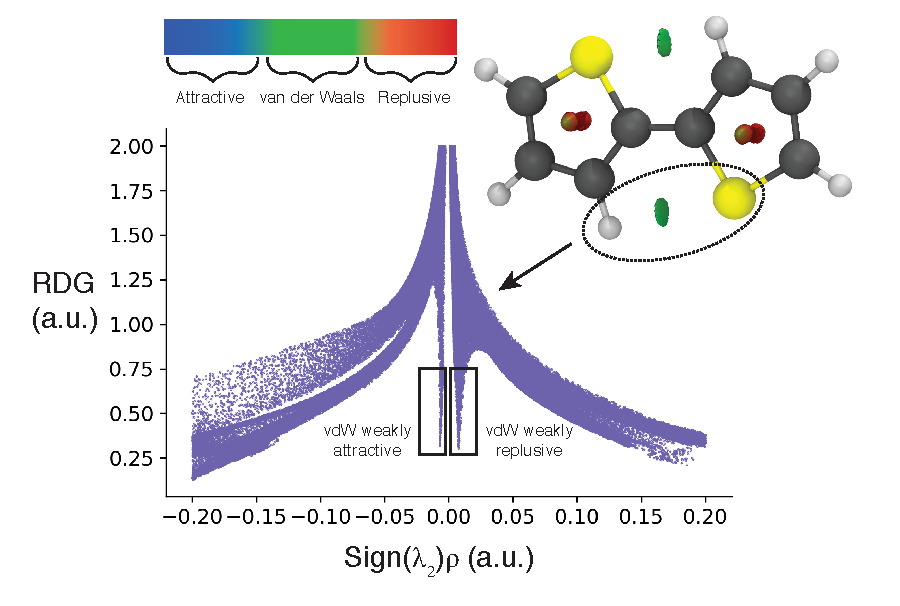
\includegraphics{figures/append_aroma/pt_nci_copy.pdf}
    \caption[\texorpdfstring{H $\cdots$ S}{HSN} NCI Analysis]{The NCI analysis of BT including an NCI isosurface (right) and an s$(\rho$) plot (center), which displays the reduced density gradient (RDG) as a function of the sign of the electron-density Hessian matrix's second eiganvalue (sign$(\lambda_{2})$) times the electron-density ($\rho$). The isosurface plot on right shows a van der Waals interaction between H $\cdots$ S. The color gradient at the top gives a rough physical description of the color scheme used for the isosurface. When only the localized region around H $\cdots$ S is considered, by employing a radius cutoff, the s$(\rho$) plot is inconclusive exhibiting both weakly repulsive and weakly attractive interactions.}
    \label{fig:pt_nci}
\end{figure}
\clearpage

\subsection{\texorpdfstring{F $\cdots$ S}{FS}}
\begin{figure}[hbt!]
    \centering
    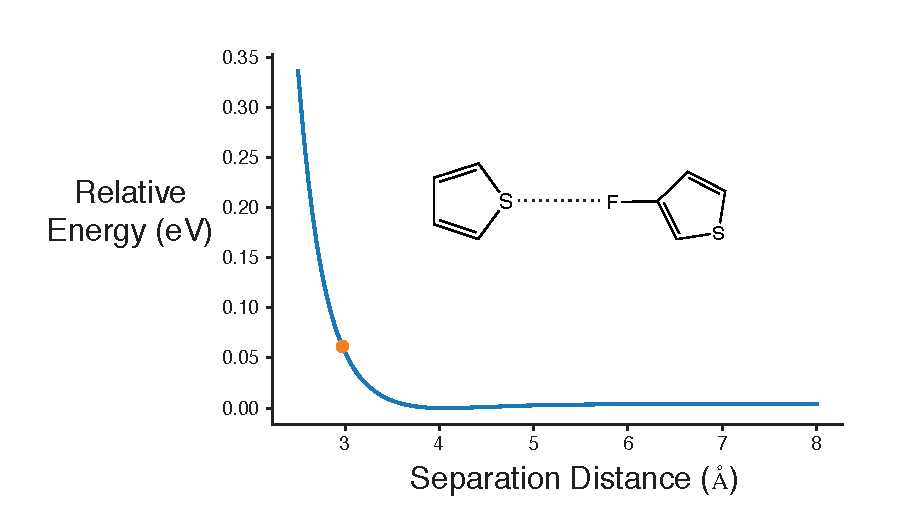
\includegraphics{figures/append_aroma/ts_t_t_f1_copy.pdf}
    \caption[\texorpdfstring{F $\cdots$ S}{FS} 1F Through-space Calculation]{A potential energy scan of the interatomic separation distance between a fluoride and a sulfur atom on a fluorinated thiophene and a thiophene molecule. The orange dot represents the relaxed F $\cdots$ S distance on a trans (180\textdegree) 3F-BT molecule. This indicates that the F $\cdots$ S through-space interaction is repulsive in trans 3F-BT.}
    \label{fig:ts_t_t_f1}
\end{figure}

\begin{figure}[hbt!]
    \centering
    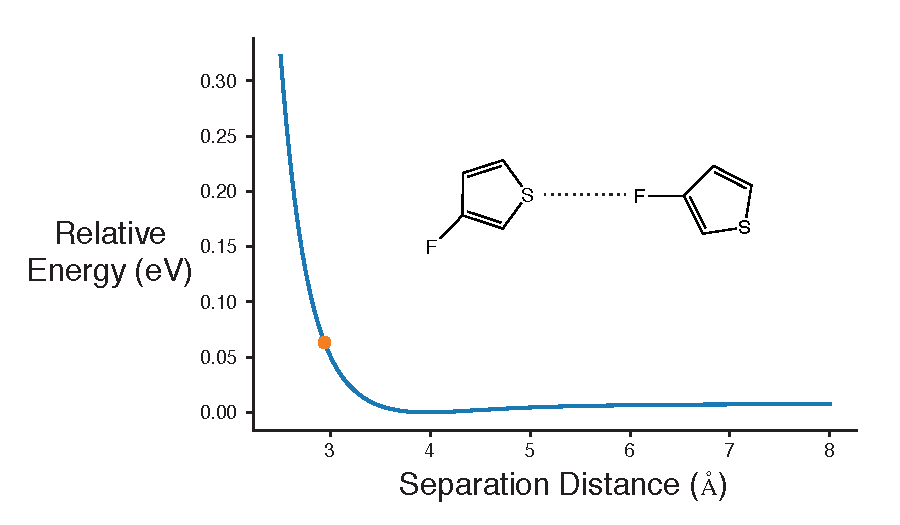
\includegraphics{figures/append_aroma/ts_2t_f1_copy.pdf}
    \caption[\texorpdfstring{F $\cdots$ S}{FS} 2F Through-space Calculation]{A potential energy scan of the interatomic separation distance between a fluoride and a sulfur atom on a fluorinated thiophene molecules. The orange dot represents the relaxed F $\cdots$ S distance on a trans (180\textdegree) F2-BT molecule. This indicates that the F $\cdots$ S through-space interaction is repulsive in trans F2-BT.}
    \label{fig:ts_2t_f1}
\end{figure}
\clearpage

\subsection{\texorpdfstring{F $\cdots$ S}{FSN} Noncovalent Interaction Analysis}
\begin{figure}[hbt!]
    \centering
    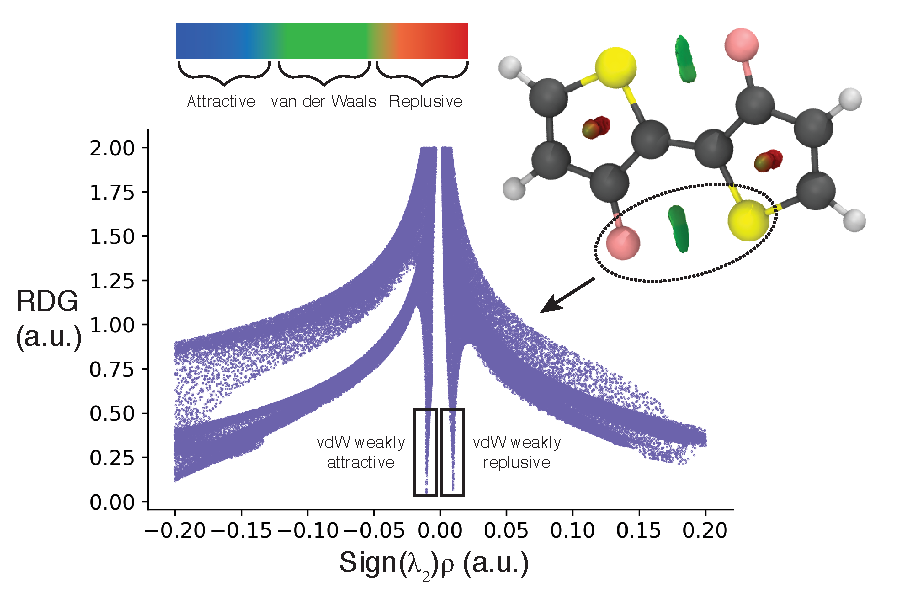
\includegraphics{figures/append_aroma/pt_f2_nciplot_copy.pdf}
    \caption[\texorpdfstring{F $\cdots$ S}{FS} NCI Analysis]{The NCI analysis of F2-BT including an NCI isosurface (right) and an s$(\rho$) plot (center), which displays the reduced density gradient (RDG) as a function of the sign of the electron-density Hessian matrix's second eiganvalue (sign$(\lambda_{2})$) times the electron-density ($\rho$). The isosurface plot on right shows a van der Waals interaction between H $\cdots$ S. The color gradient at the top gives a rough physical description of the color scheme used for the isosurface. When only the localized region around H $\cdots$ S is considered, by employing a radius cutoff, the s$(\rho$) plot is inconclusive exhibiting both weakly repulsive and weakly attractive interactions.}
    \label{fig:pt_f2_nci}
\end{figure}
\clearpage

\subsection{\texorpdfstring{O $\cdots$ S}{OS}}
\begin{figure}[hbt!]
    \centering
    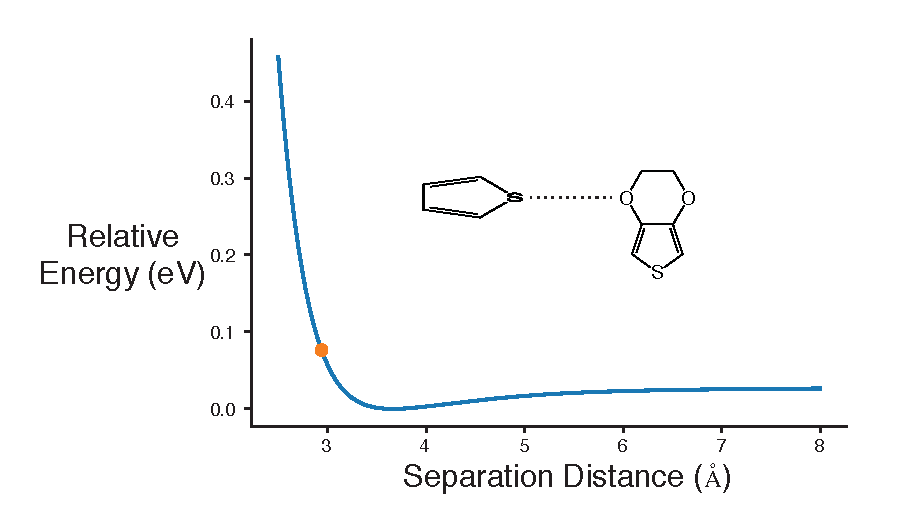
\includegraphics{figures/append_aroma/ts_t_edot_copy.pdf}
    \caption[\texorpdfstring{O $\cdots$ S}{OS} Through-space Calculation]{A potential energy scan of the interatomic separation distance between a oxygen and a sulfur atom on an EDOT and thiophene molecule respectively. The thiophene molecule has been rotated such that the ring is perpendicular to the EDOT, this is done to minimize secondary H $\cdots$ S interactions. The orange dot represents the relaxed O $\cdots$ S distance on a trans (180\textdegree) BEDOT molecule. This indicates that the O $\cdots$ S through-space interaction is repulsive in trans BEDOT.}
    \label{fig:ts_t_edot}
\end{figure}
\clearpage

\subsection{\texorpdfstring{O $\cdots$ S}{OSN} Noncovalent Interaction Analysis}
\begin{figure}[hbt!]
    \centering
    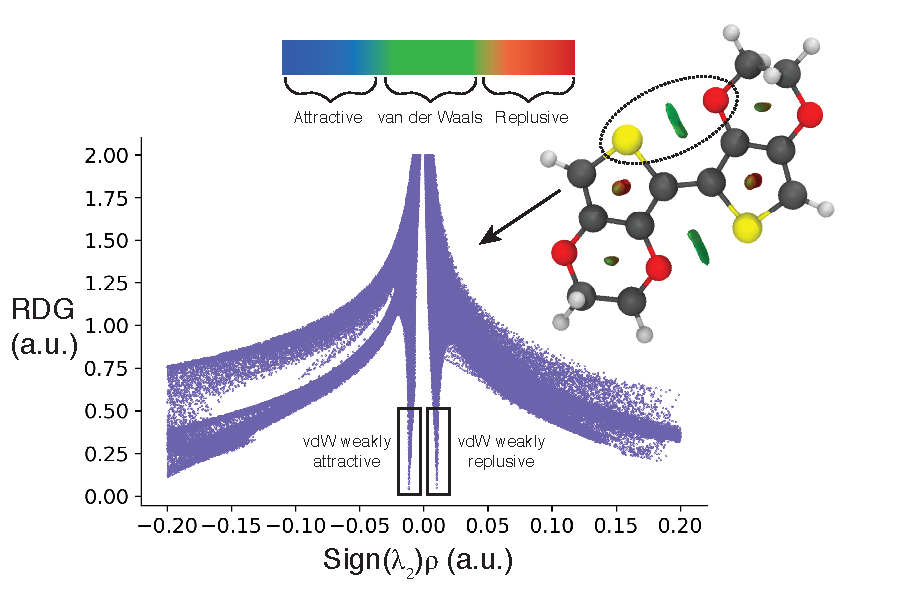
\includegraphics{figures/append_aroma/pedot_nciplot_copy.pdf}
    \caption[\texorpdfstring{O $\cdots$ S}{OSN} NCI Analysis]{The NCI analysis of BEDOT including an NCI isosurface (right) and an s$(\rho$) plot (center), which displays the reduced density gradient (RDG) as a function of the sign of the electron-density Hessian matrix's second eiganvalue (sign$(\lambda_{2})$) times the electron-density ($\rho$). The isosurface plot on right shows a van der Waals interaction between H $\cdots$ S. The color gradient at the top gives a rough physical description of the color scheme used for the isosurface. When only the localized region around H $\cdots$ S is considered, by employing a radius cutoff, the s$(\rho$) plot is inconclusive exhibiting both weakly repulsive and weakly attractive interactions.}
    \label{fig:pedot_nci}
\end{figure}
\clearpage

%%%%%%%%%%%%%%%%%%%%%%%%%%
\section{NBO Perturbation Analysis}\label{sec:aroma_nbo_e2}

\begin{table}[hbt!]\centering
\caption{NBO Stabilization Energies}
\label{tab:tpm_vals}
\renewcommand{\arraystretch}{1.5}
\begin{threeparttable}
\begin{tabular}{cccc}\toprule
\multicolumn{1}{c}{\multirow{2}{2.5cm}{\centering }} &
\multicolumn{1}{c}{\multirow{2}{1.5cm}{\centering Donor}} &
\multicolumn{1}{c}{\multirow{2}{1.6cm}{\centering Acceptor}} &
\multicolumn{1}{c}{\multirow{2}{5.5cm}{\centering Stabilization Energy E(2) \\ kcal/mol}} \\ \\ \midrule
    F2-BT\tnote{$\dagger$} & $LP_F$ & $\sigma^{*}_{C-S}$ & 0.84\\
    BEDOT\tnote{$\dagger$} & $LP_O$ & $\sigma^{*}_{C-S}$ & 1.09\\ \bottomrule
\end{tabular}
\begin{tablenotes}
\item[$\dagger$] \footnotesize Energy values represent 180\textdegree \ configurations
\end{tablenotes}
\end{threeparttable}
\end{table}

%%%%%%%%%%%%%%%%%%%%%%%%%%
\section{Expanded Methods}\label{sec:aroma_exp_method}

\subsection{Hydrogenation of BT}
Additional torsional constraints were placed on the hBT dimer during geometry optimizations to prevent ring distortion. The intent of hydrogenation was to remove aromaticity, while maintaining conjugation across the central C-C bond between rings. Ring distortion is an unintended consequence of hydrogenation and does not represent the physics of interest. As a result, the intra-ring C-C-C-C torsion angle for each thiophene ring was fixed at its undistorted state (roughly 0\textdegree), in addition to the central inter-ring C-C-C-C torsion angle being fixed at the desired angle within the potential energy scan. In sum, geometry optimizations for the hBT dimer had 3 torsional constraints, 2 intra-ring and 1 inter-ring, whereas all other degrees of freedom were allowed to relax.

\subsection{NICS Calculations}
NICS values were computed by placing fictitious hydrogen atoms (designated H-Bq in Gaussian) 1\si{\angstrom} above the center of each ring, followed by an NMR calculation with Gaussian16 \cite{g16}. The largest eigenvalue of the magnetic shielding tensor for the fictitious H atom was taken as the NICS $1_{ZZ}$ value in ppm. Conventionally, the sign of NICS values are reversed for comparison with experimental NMR values. In this work we do not reverse the sign and report the absolute NICS $1_{ZZ}$ value ($\abs*{NICS 1_{ZZ}}$) for easy comparison with MCI aromaticity values. Specific details on the NICS method have been described elsewhere \cite{Fallah-Bagher-Shaidaei2006, Chen2005}.

\subsection{Through-space Calculations}
All through-space potential energy scans utilized counterpoise corrected energies as implementation in Gaussian16. Methodology of through-space calculations has been described by others \cite{Jackson2013}.

\subsection{NCI Analysis}
NCI analysis was preformed with NCIplot \cite{Johnson2010, Contreras-Garcia2011}. The only deviation from standard procedure was adding a radius cutoff to investigate local interactions (i.e. X $\cdots$ S). For these calculations a point was specified roughly half way between the two atoms with a radius cutoff of 2\AA.

\clearpage
%%%%%%%%%%%%%%%%%%%%%%%%%%
\section{Tabular Data}

\subsection{BT}
%\subsubsection{Energy, Aromaticity, and Conjugation Data}
\begin{table}[hbt!]\centering
\caption{Bithiophene Torsional Data}
\renewcommand{\arraystretch}{1.5}
\begin{threeparttable}
\begin{tabular}{cccccc}\toprule
\multicolumn{1}{c}{\multirow{2}{2.0cm}{\centering Torsion \\ Angle (\textdegree)}} &
\multicolumn{1}{c}{\multirow{2}{2.2cm}{\centering Rel. Energy (eV)}} &
\multicolumn{1}{c}{\multirow{2}{2.5cm}{\centering Abs. Energy \\ (Hartree)}} &
\multicolumn{1}{c}{\multirow{2}{1.5cm}{\centering MCI $\times 10^3$}\tnote{$\dagger$}} &
\multicolumn{1}{c}{\multirow{2}{1.5cm}{\centering $\abs*{\bfrac{NICS} {1_{ZZ}}}$}\tnote{$\ddagger$}} &
\multicolumn{1}{c}{\multirow{2}{2.5cm}{\centering Central Bond \\ Length (\AA)}}
\\ \\ \midrule
    0.0 & 0.04106 & -1104.84898 & 66.19 (66.18) & 24.24 (24.24) & 1.455 \\
    10.0 & 0.03557 & -1104.84919 & 66.30 (66.32) & 24.53 (24.50) & 1.455 \\
    20.0 & 0.02465 & -1104.84959 & 66.69 (66.67) & 25.15 (25.14) & 1.454 \\
    30.0 & 0.01742 & -1104.84985 & 67.25 (67.25) & 25.85 (25.84) & 1.455 \\
    40.0 & 0.01849 & -1104.84981 & 67.96 (67.98) & 26.48 (26.48) & 1.456 \\
    50.0 & 0.02854 & -1104.84944 & 68.83 (68.82) & 27.03 (27.04) & 1.458 \\
    60.0 & 0.04480 & -1104.84885 & 69.83 (69.82) & 27.48 (27.48) & 1.460 \\
    70.0 & 0.06250 & -1104.84820 & 70.80 (70.77) & 27.83 (27.82) & 1.463 \\
    80.0 & 0.07593 & -1104.84770 & 71.54 (71.53) & 28.09 (28.08) & 1.465 \\
    90.0 & 0.07962 & -1104.84757 & 71.88 (71.87) & 28.25 (28.26) & 1.466 \\
    100.0 & 0.07169 & -1104.84786 & 71.60 (71.60) & 28.27 (28.28) & 1.465 \\
    110.0 & 0.05443 & -1104.84849 & 70.81 (70.83) & 28.08 (28.09) & 1.463 \\
    120.0 & 0.03391 & -1104.84925 & 69.80 (69.79) & 27.70 (27.72) & 1.460 \\
    130.0 & 0.01566 & -1104.84992 & 68.71 (68.72) & 27.14 (27.16) & 1.458 \\
    140.0 & 0.00386 & -1104.85035 & 67.71 (67.71) & 26.44 (26.45) & 1.456 \\
    150.0 & 0.00000 & -1104.85049 & 66.82 (66.82) & 25.64 (25.66) & 1.454 \\
    160.0 & 0.00284 & -1104.85039 & 66.12 (66.11) & 24.82 (24.83) & 1.454 \\
    170.0 & 0.00864 & -1104.85018 & 65.61 (65.60) & 24.15 (24.15) & 1.454 \\
    180.0 & 0.01147 & -1104.85007 & 65.42 (65.43) & 23.88 (23.88) & 1.454 \\ \bottomrule
\end{tabular}
\begin{tablenotes}
\item[*] \footnotesize All quantum calculations employed the $\omega$B97x-D functional with the def2-TZVPP basis set.
\item [$\dagger$] \footnotesize The MCI values in parentheses represent the second ring in the dimer molecule.
\item [$\ddagger$] \footnotesize The units of NICS values are ppm, and for comparison with MCI we have not reversed the sign. The NICS values in parentheses represent the second ring in the dimer molecule.
\end{tablenotes}
\end{threeparttable}
\end{table}

%\subsubsection{Relaxed Structure}
\begin{table}[hbt!]\centering
\caption{Bithiophene Relaxed Structure}
\renewcommand{\arraystretch}{1.5}
\begin{threeparttable}
\begin{tabular}{ccccc}\toprule
{} & {Atom} & {x (\AA)} & {y (\AA)} & {z (\AA)} \\ \midrule
    1 & S & 0.001 & -0.024 & -0.030\\
    2 & C & 1.708 & -0.014 & -0.014\\
    3 & H & 2.244 & -0.025 & 0.920\\
    4 & C & 2.219 & 0.008 & -1.274\\
    5 & H & 3.277 & 0.017 & -1.488\\
    6 & C & 1.210 & 0.029 & -2.269\\
    7 & H & 1.409 & 0.069 & -3.330\\
    8 & C & -0.054 & 0.021 & -1.750\\
    9 & C & -1.326 & 0.042 & -2.457\\
    10 & C & -2.520 & 0.567 & -2.048\\
    11 & H & -2.646 & 1.070 & -1.100\\
    12 & C & -3.553 & 0.408 & -3.004\\
    13 & H & -4.563 & 0.763 & -2.865\\
    14 & C & -3.130 & -0.234 & -4.126\\
    15 & H & -3.701 & -0.478 & -5.006\\
    16 & S & -1.481 & -0.662 & -4.020\\ \bottomrule
\end{tabular}
\begin{tablenotes}
\item[*] \footnotesize Level of theory: $\omega$B97x-D \\ Basis set: def2-TZVPP
\end{tablenotes}
\end{threeparttable}
\end{table}

\clearpage
\subsection{hBT}

\begin{table}[hbt!]\centering
\caption{Hydrogenated Bithiophene Torsional Data}
\renewcommand{\arraystretch}{1.5}
\begin{threeparttable}
\begin{tabular}{cccccc}\toprule
\multicolumn{1}{c}{\multirow{2}{2.0cm}{\centering Torsion \\ Angle (\textdegree)}} &
\multicolumn{1}{c}{\multirow{2}{2.2cm}{\centering Rel. Energy (eV)}} &
\multicolumn{1}{c}{\multirow{2}{2.5cm}{\centering Abs. Energy \\ (Hartree)}} &
\multicolumn{1}{c}{\multirow{2}{1.5cm}{\centering MCI $\times 10^3$}\tnote{$\dagger$}} &
\multicolumn{1}{c}{\multirow{2}{1.5cm}{\centering $\abs*{\bfrac{NICS} {1_{ZZ}}}$}\tnote{$\ddagger$}} &
\multicolumn{1}{c}{\multirow{2}{2.5cm}{\centering Central Bond \\ Length (\AA)}}
\\ \\ \midrule
0.0 & 0.16920 & -1107.25114 & 3.16 (3.16) & 4.38 (4.37) & 1.468 \\
10.0 & 0.15361 & -1107.25172 & 3.15 (3.15) & 4.53 (4.54) & 1.467 \\
20.0 & 0.12613 & -1107.25273 & 3.15 (3.15) & 4.45 (4.45) & 1.465 \\
30.0 & 0.10310 & -1107.25357 & 3.16 (3.16) & 4.30 (4.29) & 1.463 \\
40.0 & 0.09123 & -1107.25401 & 3.17 (3.17) & 4.15 (4.15) & 1.462 \\
50.0 & 0.09212 & -1107.25398 & 3.18 (3.18) & 4.01 (4.01) & 1.463 \\
60.0 & 0.10437 & -1107.25353 & 3.19 (3.19) & 3.88 (3.87) & 1.464 \\
70.0 & 0.12360 & -1107.25282 & 3.20 (3.20) & 3.74 (3.73) & 1.466 \\
80.0 & 0.14340 & -1107.25209 & 3.20 (3.20) & 3.62 (3.60) & 1.469 \\
90.0 & 0.15647 & -1107.25161 & 3.21 (3.21) & 3.53 (3.51) & 1.471 \\
100.0 & 0.15718 & -1107.25158 & 3.20 (3.20) & 3.51 (3.49) & 1.472 \\
110.0 & 0.14297 & -1107.25211 & 3.19 (3.19) & 3.59 (3.57) & 1.471 \\
120.0 & 0.11631 & -1107.25309 & 3.18 (3.18) & 3.72 (3.71) & 1.469 \\
130.0 & 0.08418 & -1107.25427 & 3.16 (3.16) & 3.86 (3.86) & 1.465 \\
140.0 & 0.05374 & -1107.25539 & 3.15 (3.15) & 4.00 (3.99) & 1.462 \\
150.0 & 0.02927 & -1107.25629 & 3.13 (3.13) & 4.13 (4.12) & 1.459 \\
160.0 & 0.01226 & -1107.25691 & 3.12 (3.12) & 4.25 (4.25) & 1.457 \\
170.0 & 0.00288 & -1107.25725 & 3.11 (3.11) & 4.37 (4.36) & 1.456 \\
180.0 & 0.00000 & -1107.25736 & 3.11 (3.11) & 4.43 (4.43) & 1.455 \\ \bottomrule
\end{tabular}
\begin{tablenotes}
\item[*] \footnotesize All quantum calculations employed the $\omega$B97x-D functional with the def2-TZVPP basis set.
\item [$\dagger$] \footnotesize The MCI values in parentheses represent the second ring in the dimer molecule.
\item [$\ddagger$] \footnotesize The units of NICS values are ppm, and for comparison with MCI we have not reversed the sign. The NICS values in parentheses represent the second ring in the dimer molecule.
\end{tablenotes}
\end{threeparttable}
\end{table}

\begin{table}[hbt!]\centering
\caption{Hydrogenated Bithiophene Relaxed Structure}
\renewcommand{\arraystretch}{1.5}
\begin{threeparttable}
\begin{tabular}{ccccc}\toprule
{} & {Atom} & {x (\AA)} & {y (\AA)} & {z (\AA)} \\ \midrule
    1 & S & -0.040 & 0.163 & 0.023\\
    2 & C & 1.764 & 0.408 & -0.006\\
    3 & C & 2.271 & -0.288 & -1.271\\
    4 & C & 1.149 & -0.217 & -2.264\\
    5 & H & 1.308 & -0.366 & -3.324\\
    6 & C & -0.061 & -0.024 & -1.739\\
    7 & C & -1.330 & -0.001 & -2.449\\
    8 & C & -2.521 & 0.341 & -1.955\\
    9 & H & -2.656 & 0.665 & -0.932\\
    10 & C & -3.675 & 0.172 & -2.898\\
    11 & C & -3.075 & 0.163 & -4.306\\
    12 & S & -1.396 & -0.522 & -4.142\\
    13 & H & 3.183 & 0.186 & -1.635\\
    14 & H & 2.513 & -1.337 & -1.068\\
    15 & H & 1.963 & 1.478 & -0.047\\
    16 & H & 2.193 & 0.003 & 0.906\\
    17 & H & -3.641 & -0.444 & -5.008\\
    18 & H & -2.994 & 1.176 & -4.699\\
    19 & H & -4.185 & -0.774 & -2.686\\
    20 & H & -4.417 & 0.965 & -2.798\\
 \bottomrule
\end{tabular}
\begin{tablenotes}
\item[*] \footnotesize Level of theory: $\omega$B97x-D \\ Basis set: def2-TZVPP
\end{tablenotes}
\end{threeparttable}
\end{table}

\clearpage
\subsection{F2-BT}

\begin{table}[hbt!]\centering
\caption{F2-BT Torsional Data}
\renewcommand{\arraystretch}{1.5}
\begin{threeparttable}
\begin{tabular}{cccccc}\toprule
\multicolumn{1}{c}{\multirow{2}{2.0cm}{\centering Torsion \\ Angle (\textdegree)}} &
\multicolumn{1}{c}{\multirow{2}{2.2cm}{\centering Rel. Energy (eV)}} &
\multicolumn{1}{c}{\multirow{2}{2.5cm}{\centering Abs. Energy \\ (Hartree)}} &
\multicolumn{1}{c}{\multirow{2}{1.5cm}{\centering MCI $\times 10^3$}\tnote{$\dagger$}} &
\multicolumn{1}{c}{\multirow{2}{1.5cm}{\centering $\abs*{\bfrac{NICS} {1_{ZZ}}}$}\tnote{$\ddagger$}} &
\multicolumn{1}{c}{\multirow{2}{2.5cm}{\centering Central Bond \\ Length (\AA)}}
\\ \\ \midrule
0.0 & 0.13549 & -1303.34351 & 56.68 (56.66) & 21.67 (21.66) & 1.455 \\
10.0 & 0.11315 & -1303.34433 & 57.03 (57.03) & 22.31 (22.31) & 1.453 \\
20.0 & 0.07472 & -1303.34574 & 57.71 (57.73) & 23.11 (23.11) & 1.452 \\
30.0 & 0.04179 & -1303.34695 & 58.51 (58.51) & 23.78 (23.78) & 1.451 \\
40.0 & 0.02160 & -1303.34770 & 59.43 (59.43) & 24.31 (24.31) & 1.451 \\
50.0 & 0.01574 & -1303.34791 & 60.37 (60.36) & 24.72 (24.72) & 1.452 \\
60.0 & 0.02076 & -1303.34773 & 61.36 (61.35) & 25.03 (25.03) & 1.454 \\
70.0 & 0.03013 & -1303.34738 & 62.22 (62.23) & 25.27 (25.27) & 1.456 \\
80.0 & 0.03786 & -1303.34710 & 62.88 (62.88) & 25.42 (25.42) & 1.457 \\
90.0 & 0.04052 & -1303.34700 & 63.21 (63.21) & 25.51 (25.51) & 1.458 \\
100.0 & 0.03844 & -1303.34708 & 63.21 (63.20) & 25.49 (25.49) & 1.458 \\
110.0 & 0.03382 & -1303.34725 & 62.95 (62.95) & 25.35 (25.35) & 1.457 \\
120.0 & 0.02904 & -1303.34742 & 62.50 (62.49) & 25.11 (25.11) & 1.455 \\
130.0 & 0.02505 & -1303.34757 & 61.91 (61.92) & 24.75 (24.75) & 1.454 \\
140.0 & 0.02163 & -1303.34769 & 61.25 (61.24) & 24.35 (24.35) & 1.453 \\
150.0 & 0.01725 & -1303.34786 & 60.48 (60.48) & 23.98 (23.98) & 1.451 \\
160.0 & 0.01002 & -1303.34812 & 59.80 (59.80) & 23.76 (23.76) & 1.450 \\
170.0 & 0.00297 & -1303.34838 & 59.30 (59.29) & 23.71 (23.71) & 1.449 \\
180.0 & 0.00000 & -1303.34849 & 59.13 (59.13) & 23.75 (23.75) & 1.449 \\ \bottomrule
\end{tabular}
\begin{tablenotes}
\item[*] \footnotesize All quantum calculations employed the $\omega$B97x-D functional with the def2-TZVPP basis set.
\item [$\dagger$] \footnotesize The MCI values in parentheses represent the second ring in the dimer molecule.
\item [$\ddagger$] \footnotesize The units of NICS values are ppm, and for comparison with MCI we have not reversed the sign. The NICS values in parentheses represent the second ring in the dimer molecule.
\end{tablenotes}
\end{threeparttable}
\end{table}

\begin{table}[hbt!]\centering
\caption{F2-BT Relaxed Structure}
\renewcommand{\arraystretch}{1.5}
\begin{threeparttable}
\begin{tabular}{ccccc}\toprule
{} & {Atom} & {x (\AA)} & {y (\AA)} & {z (\AA)} \\ \midrule
    1 & S & 0.037 & -0.486 & -0.078\\
    2 & C & 1.727 & -0.266 & -0.036\\
    3 & H & 2.270 & -0.443 & 0.877\\
    4 & C & 2.227 & 0.132 & -1.235\\
    5 & H & 3.265 & 0.332 & -1.445\\
    6 & C & 1.196 & 0.254 & -2.189\\
    7 & F & 1.446 & 0.634 & -3.445\\
    8 & C & -0.062 & -0.040 & -1.745\\
    9 & C & -1.307 & -0.007 & -2.484\\
    10 & C & -2.565 & -0.304 & -2.040\\
    11 & F & -2.815 & -0.686 & -0.785\\
    12 & C & -3.596 & -0.181 & -2.994\\
    13 & H & -4.634 & -0.382 & -2.784\\
    14 & C & -3.097 & 0.220 & -4.192\\
    15 & H & -3.639 & 0.399 & -5.105\\
    16 & S & -1.406 & 0.441 & -4.150\\ \bottomrule
\end{tabular}
\begin{tablenotes}
\item[*] \footnotesize Level of theory: $\omega$B97x-D \\ Basis set: def2-TZVPP
\end{tablenotes}
\end{threeparttable}
\end{table}

\begin{table}[hbt!]\centering
\caption{F2-BT RHF and RHF NBO Deletion Energies}
\renewcommand{\arraystretch}{1.5}
\begin{threeparttable}
\begin{tabular}{ccccc}\toprule
\multirow{1}{*}{} & \multicolumn{2}{c}{RHF} & \multicolumn{2}{c}{RHF Deletion\tnote{$\dagger$}} \\
\midrule
\multicolumn{1}{c}{\multirow{2}{2.0cm}{\centering Torsion Angle (\textdegree)}} &
\multicolumn{1}{c}{\multirow{2}{2.2cm}{\centering Rel. Energy (eV)}} &
\multicolumn{1}{c}{\multirow{2}{2.5cm}{\centering Abs. Energy (Hartree)}} &
\multicolumn{1}{c}{\multirow{2}{2.2cm}{\centering Rel. Energy (eV)}} &
\multicolumn{1}{c}{\multirow{2}{2.5cm}{\centering Abs. Energy (Hartree)}}
\\ \\\midrule
0.0 & 0.13996 & -1299.37850 & 0.16754 & -1299.35295 \\
10.0 & 0.11538 & -1299.37940 & 0.13726 & -1299.35406 \\
20.0 & 0.07148 & -1299.38101 & 0.08629 & -1299.35593 \\
30.0 & 0.03270 & -1299.38244 & 0.04196 & -1299.35756 \\
40.0 & 0.00841 & -1299.38333 & 0.01336 & -1299.35861 \\
50.0 & 0.00000 & -1299.38364 & 0.00116 & -1299.35906 \\
60.0 & 0.00259 & -1299.38354 & 0.00000 & -1299.35910 \\
70.0 & 0.00899 & -1299.38331 & 0.00320 & -1299.35899 \\
80.0 & 0.01411 & -1299.38312 & 0.00638 & -1299.35887 \\
90.0 & 0.01607 & -1299.38305 & 0.00783 & -1299.35882 \\
100.0 & 0.01536 & -1299.38307 & 0.00735 & -1299.35883 \\
110.0 & 0.01359 & -1299.38314 & 0.00606 & -1299.35888 \\
120.0 & 0.01250 & -1299.38318 & 0.00567 & -1299.35890 \\
130.0 & 0.01301 & -1299.38316 & 0.00796 & -1299.35881 \\
140.0 & 0.01444 & -1299.38311 & 0.01437 & -1299.35858 \\
150.0 & 0.01453 & -1299.38311 & 0.02579 & -1299.35816 \\
160.0 & 0.01131 & -1299.38322 & 0.04070 & -1299.35761 \\
170.0 & 0.00639 & -1299.38340 & 0.05317 & -1299.35715 \\
180.0 & 0.00405 & -1299.38349 & 0.05803 & -1299.35697 \\ \bottomrule
\end{tabular}
\begin{tablenotes}
\item[*] \footnotesize All quantum calculations employed the restricted Hartree-Fock (RHF) level of theory with the def2-TZVPP basis set.
\item[$\dagger$] \footnotesize NBO6 and Gaussian09 were used to delete both $\sigma^{*}_{C-S}$ orbitals from the Fock matrix and calculate the corresponding energy.
\end{tablenotes}
\end{threeparttable}
\end{table}

\clearpage
\subsection{BEDOT}

\begin{table}[hbt!]\centering
\caption{BEDOT Torsional Data}
\renewcommand{\arraystretch}{1.5}
\begin{threeparttable}
\begin{tabular}{cccccc}\toprule
\multicolumn{1}{c}{\multirow{2}{2.0cm}{\centering Torsion \\ Angle (\textdegree)}} &
\multicolumn{1}{c}{\multirow{2}{2.2cm}{\centering Rel. Energy (eV)}} &
\multicolumn{1}{c}{\multirow{2}{2.5cm}{\centering Abs. Energy \\ (Hartree)}} &
\multicolumn{1}{c}{\multirow{2}{1.5cm}{\centering MCI $\times 10^3$}\tnote{$\dagger$}} &
\multicolumn{1}{c}{\multirow{2}{1.5cm}{\centering $\abs*{\bfrac{NICS} {1_{ZZ}}}$}\tnote{$\ddagger$}} &
\multicolumn{1}{c}{\multirow{2}{2.5cm}{\centering Central Bond \\ Length (\AA)}}
\\ \\ \midrule
0.0 & 0.22303 & -1560.56546 & 44.17 (44.18) & 19.73 (19.70) & 1.457 \\
10.0 & 0.18094 & -1560.56701 & 44.62 (44.61) & 20.68 (20.66) & 1.453 \\
20.0 & 0.12507 & -1560.56906 & 45.26 (45.24) & 21.50 (21.46) & 1.451 \\
30.0 & 0.07837 & -1560.57078 & 45.98 (45.97) & 22.15 (22.14) & 1.450 \\
40.0 & 0.04952 & -1560.57184 & 46.75 (46.75) & 22.65 (22.66) & 1.450 \\
50.0 & 0.04054 & -1560.57217 & 47.54 (47.57) & 23.04 (23.04) & 1.451 \\
60.0 & 0.04721 & -1560.57192 & 48.36 (48.35) & 23.36 (23.37) & 1.453 \\
70.0 & 0.06129 & -1560.57140 & 49.12 (49.13) & 23.59 (23.61) & 1.455 \\
80.0 & 0.07344 & -1560.57096 & 49.66 (49.66) & 23.74 (23.76) & 1.457 \\
90.0 & 0.07919 & -1560.57075 & 49.86 (49.87) & 23.80 (23.82) & 1.457 \\
100.0 & 0.07864 & -1560.57077 & 49.81 (49.82) & 23.74 (23.76) & 1.457 \\
110.0 & 0.07479 & -1560.57091 & 49.55 (49.55) & 23.56 (23.57) & 1.456 \\
120.0 & 0.06940 & -1560.57111 & 49.18 (49.18) & 23.28 (23.28) & 1.455 \\
130.0 & 0.06277 & -1560.57135 & 48.70 (48.71) & 22.92 (22.92) & 1.453 \\
140.0 & 0.05341 & -1560.57169 & 48.12 (48.15) & 22.57 (22.58) & 1.452 \\
150.0 & 0.03956 & -1560.57220 & 47.46 (47.47) & 22.36 (22.37) & 1.450 \\
160.0 & 0.02210 & -1560.57284 & 46.78 (46.78) & 22.30 (22.30) & 1.448 \\
170.0 & 0.00637 & -1560.57342 & 46.31 (46.33) & 22.31 (22.31) & 1.447 \\
180.0 & 0.00000 & -1560.57366 & 46.17 (46.16) & 22.31 (22.30) & 1.447 \\ \bottomrule
\end{tabular}
\begin{tablenotes}
\item[*] \footnotesize All quantum calculations employed the $\omega$B97x-D functional with the def2-TZVPP basis set.
\item [$\dagger$] \footnotesize The MCI values in parentheses represent the second ring in the dimer molecule.
\item [$\ddagger$] \footnotesize The units of NICS values are ppm, and for comparison with MCI we have not reversed the sign. The NICS values in parentheses represent the second ring in the dimer molecule.
\end{tablenotes}
\end{threeparttable}
\end{table}

\begin{table}[hbt!]\centering
\caption{BEDOT Relaxed Structure}
\renewcommand{\arraystretch}{1.25}
\begin{threeparttable}
\begin{tabular}{ccccc}\toprule
{} & {Atom} & {x (\AA)} & {y (\AA)} & {z (\AA)} \\ \midrule
    1 & S & 0.212 & -0.710 & -0.167\\
    2 & C & 1.900 & -0.439 & -0.177\\
    3 & H & 2.495 & -0.581 & 0.709\\
    4 & C & 2.326 & -0.036 & -1.400\\
    5 & C & 1.269 & 0.050 & -2.346\\
    6 & C & 0.043 & -0.282 & -1.835\\
    7 & C & -1.226 & -0.307 & -2.529\\
    8 & C & -2.452 & -0.637 & -2.018\\
    9 & C & -3.507 & -0.570 & -2.969\\
    10 & C & -3.076 & -0.196 & -4.200\\
    11 & H & -3.668 & -0.069 & -5.090\\
    12 & S & -1.389 & 0.082 & -4.208\\
    13 & O & 3.615 & 0.245 & -1.723\\
    14 & O & 1.472 & 0.443 & -3.630\\
    15 & C & 3.723 & 0.974 & -2.936\\
    16 & C & 2.838 & 0.375 & -4.009\\
    17 & H & 4.768 & 0.928 & -3.234\\
    18 & H & 3.445 & 2.019 & -2.765\\
    19 & H & 2.930 & 0.933 & -4.938\\
    20 & H & 3.118 & -0.668 & -4.187\\
    21 & O & -4.792 & -0.873 & -2.652\\
    22 & O & -2.663 & -0.982 & -0.722\\
    23 & C & -5.017 & -0.878 & -1.251\\
    24 & C & -3.915 & -1.622 & -0.527\\
    25 & H & -4.096 & -1.629 & 0.545\\
    26 & H & -3.859 & -2.654 & -0.889\\
    27 & H & -5.976 & -1.366 & -1.092\\
    28 & H & -5.074 & 0.152 & -0.883\\ \bottomrule
\end{tabular}
\begin{tablenotes}
\item[*] \footnotesize Level of theory: $\omega$B97x-D \\ Basis set: def2-TZVPP
\end{tablenotes}
\end{threeparttable}
\end{table}

\begin{table}[hbt!]\centering
\caption{BEDOT RHF and RHF NBO Deletion Energies}
\renewcommand{\arraystretch}{1.5}
\begin{threeparttable}
\begin{tabular}{ccccc}\toprule
\multirow{1}{*}{} & \multicolumn{2}{c}{RHF} & \multicolumn{2}{c}{RHF Deletion\tnote{$\dagger$}} \\
\midrule
\multicolumn{1}{c}{\multirow{2}{2.0cm}{\centering Torsion Angle (\textdegree)}} &
\multicolumn{1}{c}{\multirow{2}{2.2cm}{\centering Rel. Energy (eV)}} &
\multicolumn{1}{c}{\multirow{2}{2.5cm}{\centering Abs. Energy (Hartree)}} &
\multicolumn{1}{c}{\multirow{2}{2.2cm}{\centering Rel. Energy (eV)}} &
\multicolumn{1}{c}{\multirow{2}{2.5cm}{\centering Abs. Energy (Hartree)}}
\\ \\\midrule
0.0 & 0.24056 & -1554.97676 & 0.27723 & -1554.95816 \\
10.0 & 0.19528 & -1554.97842 & 0.21892 & -1554.96030 \\
20.0 & 0.12939 & -1554.98084 & 0.14046 & -1554.96319 \\
30.0 & 0.07253 & -1554.98293 & 0.07378 & -1554.96564 \\
40.0 & 0.03418 & -1554.98434 & 0.02806 & -1554.96732 \\
50.0 & 0.01693 & -1554.98497 & 0.00498 & -1554.96817 \\
60.0 & 0.01697 & -1554.98497 & 0.00000 & -1554.96835 \\
70.0 & 0.02545 & -1554.98466 & 0.00418 & -1554.96819 \\
80.0 & 0.03364 & -1554.98436 & 0.00935 & -1554.96800 \\
90.0 & 0.03754 & -1554.98422 & 0.01187 & -1554.96791 \\
100.0 & 0.03768 & -1554.98421 & 0.01140 & -1554.96793 \\
110.0 & 0.03625 & -1554.98426 & 0.00965 & -1554.96799 \\
120.0 & 0.03520 & -1554.98430 & 0.00867 & -1554.96803 \\
130.0 & 0.03508 & -1554.98431 & 0.01027 & -1554.96797 \\
140.0 & 0.03436 & -1554.98433 & 0.01590 & -1554.96776 \\
150.0 & 0.02949 & -1554.98451 & 0.02701 & -1554.96736 \\
160.0 & 0.01838 & -1554.98492 & 0.04181 & -1554.96681 \\
170.0 & 0.00578 & -1554.98538 & 0.05353 & -1554.96638 \\
180.0 & 0.00000 & -1554.98560 & 0.05803 & -1554.96622 \\ \bottomrule
\end{tabular}
\begin{tablenotes}
\item[*] \footnotesize All quantum calculations employed the restricted Hartree-Fock (RHF) level of theory with the def2-TZVPP basis set.
\item[$\dagger$] \footnotesize NBO6 and Gaussian09 were used to delete both $\sigma^{*}_{C-S}$ orbitals from the Fock matrix and calculate the corresponding energy.
\end{tablenotes}
\end{threeparttable}
\end{table}

\clearpage
\subsection{3F-BT}

\begin{table}[hbt!]\centering
\caption{3F-BT Torsional Data}
\renewcommand{\arraystretch}{1.5}
\begin{threeparttable}
\begin{tabular}{cccccc}\toprule
\multicolumn{1}{c}{\multirow{2}{2.0cm}{\centering Torsion \\ Angle (\textdegree)}} &
\multicolumn{1}{c}{\multirow{2}{2.2cm}{\centering Rel. Energy (eV)}} &
\multicolumn{1}{c}{\multirow{2}{2.5cm}{\centering Abs. Energy \\ (Hartree)}} &
\multicolumn{1}{c}{\multirow{2}{1.5cm}{\centering MCI $\times 10^3$}\tnote{$\dagger$}} &
\multicolumn{1}{c}{\multirow{2}{1.5cm}{\centering $\abs*{\bfrac{NICS} {1_{ZZ}}}$}\tnote{$\ddagger$}} &
\multicolumn{1}{c}{\multirow{2}{2.5cm}{\centering Central Bond \\ Length (\AA)}}
\\ \\ \midrule
0.0 & 0.00895 & -1204.09895 & 58.05 (64.89) & 22.05 (24.75) & 1.452 \\
10.0 & 0.00627 & -1204.09905 & 58.21 (65.11) & 22.47 (24.98) & 1.452 \\
20.0 & 0.00159 & -1204.09922 & 58.69 (65.67) & 23.15 (25.49) & 1.452 \\
30.0 & 0.00000 & -1204.09928 & 59.28 (66.51) & 23.81 (26.05) & 1.452 \\
40.0 & 0.00442 & -1204.09912 & 60.04 (67.49) & 24.39 (26.57) & 1.454 \\
50.0 & 0.01515 & -1204.09872 & 60.85 (68.62) & 24.84 (27.03) & 1.455 \\
60.0 & 0.02952 & -1204.09820 & 61.64 (69.80) & 25.17 (27.43) & 1.458 \\
70.0 & 0.04379 & -1204.09767 & 62.38 (70.90) & 25.41 (27.74) & 1.460 \\
80.0 & 0.05374 & -1204.09731 & 62.92 (71.75) & 25.58 (27.99) & 1.462 \\
90.0 & 0.05643 & -1204.09721 & 63.12 (72.18) & 25.67 (28.15) & 1.462 \\
100.0 & 0.05146 & -1204.09739 & 62.95 (72.13) & 25.67 (28.16) & 1.462 \\
110.0 & 0.04101 & -1204.09777 & 62.45 (71.66) & 25.51 (28.01) & 1.460 \\
120.0 & 0.02875 & -1204.09822 & 61.72 (70.96) & 25.16 (27.76) & 1.458 \\
130.0 & 0.01745 & -1204.09864 & 60.86 (70.08) & 24.62 (27.41) & 1.456 \\
140.0 & 0.00919 & -1204.09894 & 59.93 (69.22) & 23.88 (27.04) & 1.454 \\
150.0 & 0.00454 & -1204.09911 & 59.03 (68.39) & 23.05 (26.67) & 1.453 \\
160.0 & 0.00247 & -1204.09919 & 58.25 (67.69) & 22.24 (26.36) & 1.452 \\
170.0 & 0.00173 & -1204.09922 & 57.69 (67.21) & 21.73 (26.11) & 1.451 \\
180.0 & 0.00170 & -1204.09922 & 57.49 (67.05) & 21.67 (25.92) & 1.451 \\ \bottomrule
\end{tabular}
\begin{tablenotes}
\item[*] \footnotesize All quantum calculations employed the $\omega$B97x-D functional with the def2-TZVPP basis set.
\item [$\dagger$] \footnotesize The MCI values in parentheses represent the second ring in the dimer molecule.
\item [$\ddagger$] \footnotesize The units of NICS values are ppm, and for comparison with MCI we have not reversed the sign. The NICS values in parentheses represent the second ring in the dimer molecule.
\end{tablenotes}
\end{threeparttable}
\end{table}

\begin{table}[hbt!]\centering
\caption{3F-BT Relaxed Structure}
\renewcommand{\arraystretch}{1.5}
\begin{threeparttable}
\begin{tabular}{ccccc}\toprule
{} & {Atom} & {x (\AA)} & {y (\AA)} & {z (\AA)} \\ \midrule
   1 & S & 0.027 & -0.481 & -0.106\\
    2 & C & 1.720 & -0.267 & -0.041\\
    3 & H & 2.251 & -0.447 & 0.878\\
    4 & C & 2.229 & 0.132 & -1.234\\
    5 & H & 3.271 & 0.330 & -1.433\\
    6 & C & 1.208 & 0.259 & -2.201\\
    7 & F & 1.475 & 0.640 & -3.452\\
    8 & C & -0.054 & -0.033 & -1.770\\
    9 & C & -1.311 & -0.006 & -2.495\\
    10 & C & -2.555 & -0.315 & -2.013\\
    11 & H & -2.733 & -0.626 & -0.994\\
    12 & C & -3.576 & -0.186 & -2.983\\
    13 & H & -4.619 & -0.385 & -2.790\\
    14 & C & -3.097 & 0.220 & -4.189\\
    15 & H & -3.648 & 0.398 & -5.097\\
    16 & S & -1.407 & 0.446 & -4.157\\ \bottomrule
\end{tabular}
\begin{tablenotes}
\item[*] \footnotesize Level of theory: $\omega$B97x-D \\ Basis set: def2-TZVPP
\end{tablenotes}
\end{threeparttable}
\end{table}

\clearpage
\subsection{4F-BT}

\begin{table}[hbt!]\centering
\caption{4F-BT Torsional Data}
\renewcommand{\arraystretch}{1.5}
\begin{threeparttable}
\begin{tabular}{cccccc}\toprule
\multicolumn{1}{c}{\multirow{2}{2.0cm}{\centering Torsion \\ Angle (\textdegree)}} &
\multicolumn{1}{c}{\multirow{2}{2.2cm}{\centering Rel. Energy (eV)}} &
\multicolumn{1}{c}{\multirow{2}{2.5cm}{\centering Abs. Energy \\ (Hartree)}} &
\multicolumn{1}{c}{\multirow{2}{1.5cm}{\centering MCI $\times 10^3$}\tnote{$\dagger$}} &
\multicolumn{1}{c}{\multirow{2}{1.5cm}{\centering $\abs*{\bfrac{NICS} {1_{ZZ}}}$}\tnote{$\ddagger$}} &
\multicolumn{1}{c}{\multirow{2}{2.5cm}{\centering Central Bond \\ Length (\AA)}}
\\ \\ \midrule
0.0 & 0.04013 & -1204.09890 & 57.89 (66.42) & 21.76 (24.38) & 1.454 \\
10.0 & 0.03445 & -1204.09911 & 58.02 (66.56) & 22.05 (24.67) & 1.454 \\
20.0 & 0.02336 & -1204.09952 & 58.38 (66.91) & 22.68 (25.35) & 1.454 \\
30.0 & 0.01622 & -1204.09978 & 58.90 (67.43) & 23.38 (26.04) & 1.454 \\
40.0 & 0.01770 & -1204.09973 & 59.60 (68.15) & 24.03 (26.68) & 1.455 \\
50.0 & 0.02851 & -1204.09933 & 60.43 (68.98) & 24.59 (27.20) & 1.457 \\
60.0 & 0.04586 & -1204.09869 & 61.39 (69.95) & 25.03 (27.60) & 1.460 \\
70.0 & 0.06472 & -1204.09800 & 62.33 (70.90) & 25.37 (27.90) & 1.462 \\
80.0 & 0.07900 & -1204.09747 & 63.11 (71.66) & 25.62 (28.11) & 1.465 \\
90.0 & 0.08278 & -1204.09733 & 63.43 (71.94) & 25.77 (28.25) & 1.465 \\
100.0 & 0.07420 & -1204.09765 & 63.17 (71.66) & 25.78 (28.26) & 1.465 \\
110.0 & 0.05592 & -1204.09832 & 62.40 (70.86) & 25.61 (28.09) & 1.462 \\
120.0 & 0.03445 & -1204.09911 & 61.40 (69.87) & 25.25 (27.76) & 1.460 \\
130.0 & 0.01557 & -1204.09980 & 60.36 (68.85) & 24.73 (27.26) & 1.457 \\
140.0 & 0.00357 & -1204.10025 & 59.40 (67.90) & 24.06 (26.62) & 1.455 \\
150.0 & 0.00000 & -1204.10038 & 58.53 (67.12) & 23.28 (25.90) & 1.454 \\
160.0 & 0.00354 & -1204.10025 & 57.84 (66.48) & 22.46 (25.10) & 1.453 \\
170.0 & 0.01018 & -1204.10000 & 57.36 (66.03) & 21.76 (24.44) & 1.453 \\
180.0 & 0.01340 & -1204.09988 & 57.15 (65.87) & 21.47 (24.15) & 1.453 \\\bottomrule
\end{tabular}
\begin{tablenotes}
\item[*] \footnotesize All quantum calculations employed the $\omega$B97x-D functional with the def2-TZVPP basis set.
\item [$\dagger$] \footnotesize The MCI values in parentheses represent the second ring in the dimer molecule.
\item [$\ddagger$] \footnotesize The units of NICS values are ppm, and for comparison with MCI we have not reversed the sign. The NICS values in parentheses represent the second ring in the dimer molecule.
\end{tablenotes}
\end{threeparttable}
\end{table}

\begin{table}[hbt!]\centering
\caption{4F-BT Relaxed Structure}
\renewcommand{\arraystretch}{1.5}
\begin{threeparttable}
\begin{tabular}{ccccc}\toprule
{} & {Atom} & {x (\AA)} & {y (\AA)} & {z (\AA)} \\ \midrule
1 & S & -0.024 & -0.016 & -0.026\\
2 & C & 1.685 & -0.031 & 0.011\\
3 & H & 2.237 & -0.073 & 0.933\\
4 & C & 2.172 & 0.019 & -1.253\\
5 & F & 3.475 & 0.024 & -1.537\\
6 & C & 1.192 & 0.056 & -2.269\\
7 & H & 1.419 & 0.072 & -3.324\\
8 & C & -0.070 & 0.034 & -1.746\\
9 & C & -1.341 & 0.053 & -2.452\\
10 & C & -2.529 & -0.510 & -2.077\\
11 & H & -2.647 & -1.081 & -1.167\\
12 & C & -3.566 & -0.292 & -3.017\\
13 & H & -4.572 & -0.664 & -2.901\\
14 & C & -3.151 & 0.431 & -4.092\\
15 & H & -3.726 & 0.732 & -4.951\\
16 & S & -1.505 & 0.863 & -3.962\\ \bottomrule
\end{tabular}
\begin{tablenotes}
\item[*] \footnotesize Level of theory: $\omega$B97x-D \\ Basis set: def2-TZVPP
\end{tablenotes}
\end{threeparttable}
\end{table}
